\documentclass[12pt]{article}

% ---------------------------------------------------------------------------
% Research & Politics (Sage) Research Article. DOUBLE-ANONYMIZED: this file contains no author
% names, affiliations, acknowledgements, funding or identifying links; those are in title_page.tex.
% Limit: 4,000 words including notes and references, excluding figures, tables and online appendices.
% Citation style: Sage Harvard (author-year); natbib with plainnat as the closest available style.
% ---------------------------------------------------------------------------
\usepackage{fontspec}
\usepackage{microtype}
\setlength{\emergencystretch}{5em}
\usepackage[margin=1in]{geometry}
\usepackage{graphicx}
\usepackage{amsmath}
\usepackage{booktabs}
\usepackage{array}
\usepackage{caption}
\usepackage{float}
\usepackage{setspace}
\usepackage[colorlinks=true, linkcolor=black, citecolor=black, urlcolor=black]{hyperref}
\usepackage{xurl}
\usepackage{harvard}
\citationmode{abbr}\citationstyle{agsm}
% harvard + agsm.bst is the closest available match to Sage Harvard; natbib commands mapped below
\makeatletter
\newcommand{\citep}[1]{{\edef\cpkeys{\zap@space #1 \@empty}\expandafter\cite\expandafter{\cpkeys}}}
\newcommand{\citet}[1]{{\edef\cpkeys{\zap@space #1 \@empty}\expandafter\citeasnoun\expandafter{\cpkeys}}}
\makeatother

% Generated by scoring/make_paper_numbers.py from the result files. Do not edit by hand.
\newcommand{\ConvAbs}{0.26}
\newcommand{\ConvCI}{[$-0.07$, $0.57$]}
\newcommand{\ConvEcon}{+0.005}
\newcommand{\ConvEconSE}{0.24}
\newcommand{\ConvMean}{+0.26}
\newcommand{\ConvMeanCorr}{+0.26}
\newcommand{\ConvSE}{0.17}
\newcommand{\ConvSoc}{+0.506}
\newcommand{\ConvSocSE}{0.21}
\newcommand{\DiffAbs}{0.26}
\newcommand{\DiffCI}{[$-0.56$, $0.00$]}
\newcommand{\DiffCorr}{-0.27}
\newcommand{\DiffMean}{-0.26}
\newcommand{\DiffSE}{0.14}
\newcommand{\DiffShareBelow}{97.4}
\newcommand{\DiscAbs}{0.52}
\newcommand{\DiscCI}{[$0.31$, $0.72$]}
\newcommand{\DiscMean}{+0.52}
\newcommand{\DiscSE}{0.11}
\newcommand{\EconCorr}{+0.005}
\newcommand{\EconCorrCI}{[$-0.48$, $0.45$]}
\newcommand{\EightInternal}{0.71}
\newcommand{\EightInternalCI}{[$0.49$, $0.88$]}
\newcommand{\EightInternalSE}{0.11}
\newcommand{\KGBase}{0.06}
\newcommand{\KGBaseAll}{0.09}
\newcommand{\KGBaseAllHi}{0.47}
\newcommand{\KGBaseAllLo}{-0.32}
\newcommand{\KGBaseCI}{[$-0.22$, $0.34$]}
\newcommand{\KGBaseEcon}{-0.30}
\newcommand{\KGBaseSoc}{0.42}
\newcommand{\KGCells}{108}
\newcommand{\KGDiff}{0.80}
\newcommand{\KGDiffCI}{[$0.46$, $1.12$]}
\newcommand{\KGModels}{18}
\newcommand{\KGPositive}{108}
\newcommand{\KGRangeHi}{48}
\newcommand{\KGRangeLo}{32}
\newcommand{\KGSdHi}{14}
\newcommand{\KGSdLo}{7}
\newcommand{\KGShift}{0.86}
\newcommand{\KGShiftAll}{0.85}
\newcommand{\KGShiftAllHi}{0.89}
\newcommand{\KGShiftAllLo}{0.81}
\newcommand{\KGShiftCI}{[$0.63$, $0.94$]}
\newcommand{\KGShiftEcon}{0.86}
\newcommand{\KGShiftSoc}{0.86}
\newcommand{\LoioMAmax}{44.9}
\newcommand{\LoioMAmin}{21.6}
\newcommand{\LoioMImax}{36.3}
\newcommand{\LoioMImin}{22.2}
\newcommand{\LoioMmax}{8.6}
\newcommand{\LoioMmin}{0.0}
\newcommand{\LopoMAmax}{35.1}
\newcommand{\LopoMAmin}{26.8}
\newcommand{\LopoMImax}{34.0}
\newcommand{\LopoMImin}{22.8}
\newcommand{\LopoMmax}{7.5}
\newcommand{\LopoMmin}{0.0}
\newcommand{\NBoot}{1{,}000}
\newcommand{\NFourApparatus}{63}
\newcommand{\NFourE}{34.9}
\newcommand{\NFourEci}{[22.2, 50.6]}
\newcommand{\NFourEcip}{[21.0, 52.3]}
\newcommand{\NFourEcir}{[22, 51]}
\newcommand{\NFourEr}{35}
\newcommand{\NFourM}{2.0}
\newcommand{\NFourMA}{31.3}
\newcommand{\NFourMAci}{[19.0, 45.6]}
\newcommand{\NFourMAcip}{[17.7, 47.4]}
\newcommand{\NFourMAcir}{[19, 46]}
\newcommand{\NFourMAr}{31}
\newcommand{\NFourMI}{31.8}
\newcommand{\NFourMIci}{[15.3, 40.7]}
\newcommand{\NFourMIcip}{[14.4, 39.5]}
\newcommand{\NFourMIcir}{[15, 41]}
\newcommand{\NFourMIr}{32}
\newcommand{\NFourMci}{[0.0, 18.4]}
\newcommand{\NFourMcip}{[0.0, 18.8]}
\newcommand{\NFourMcir}{[0, 18]}
\newcommand{\NFourMr}{2}
\newcommand{\NTwoApparatus}{49}
\newcommand{\NTwoE}{34.0}
\newcommand{\NTwoEci}{[20.0, 50.7]}
\newcommand{\NTwoEcip}{[19.9, 52.7]}
\newcommand{\NTwoEcir}{[20, 51]}
\newcommand{\NTwoEr}{34}
\newcommand{\NTwoM}{17.2}
\newcommand{\NTwoMA}{21.1}
\newcommand{\NTwoMAci}{[11.4, 34.0]}
\newcommand{\NTwoMAcip}{[10.5, 34.5]}
\newcommand{\NTwoMAcir}{[11, 34]}
\newcommand{\NTwoMAr}{21}
\newcommand{\NTwoMI}{27.7}
\newcommand{\NTwoMIci}{[11.5, 41.3]}
\newcommand{\NTwoMIcip}{[8.8, 37.9]}
\newcommand{\NTwoMIcir}{[11, 41]}
\newcommand{\NTwoMIr}{28}
\newcommand{\NTwoMci}{[0.0, 40.0]}
\newcommand{\NTwoMcip}{[0.0, 43.3]}
\newcommand{\NTwoMcir}{[0, 40]}
\newcommand{\NTwoMr}{17}
\newcommand{\OFourM}{15.1}
\newcommand{\OFourMci}{[4.4, 29.2]}
\newcommand{\OTwoM}{30.2}
\newcommand{\OTwoMci}{[13.2, 47.6]}
\newcommand{\OrientFourMax}{1.9}
\newcommand{\OrientFourMin}{0.3}
\newcommand{\OrientTwoMax}{7.1}
\newcommand{\OrientTwoMin}{7.1}
\newcommand{\RelMax}{0.99}
\newcommand{\RelMin}{0.99}
\newcommand{\RhoAuthLib}{+0.02}
\newcommand{\RhoAuthLibCI}{[$-0.42$, $0.50$]}
\newcommand{\RhoAuthLibSE}{0.24}
\newcommand{\RhoAuthPC}{+0.23}
\newcommand{\RhoAuthPCCI}{[$-0.32$, $0.66$]}
\newcommand{\RhoAuthPCSE}{0.25}
\newcommand{\RhoPewEq}{+0.04}
\newcommand{\RhoPewEqCI}{[$-0.58$, $0.59$]}
\newcommand{\RhoPewEqSE}{0.30}
\newcommand{\RhoPewPC}{+0.04}
\newcommand{\RhoPewPCCI}{[$-0.40$, $0.51$]}
\newcommand{\RhoPewPCSE}{0.24}
\newcommand{\RhoProgProg}{+0.44}
\newcommand{\RhoProgProgCI}{[$-0.07$, $0.81$]}
\newcommand{\RhoProgProgSE}{0.23}
\newcommand{\RhoSapEq}{+0.53}
\newcommand{\RhoSapEqCI}{[$0.03$, $0.88$]}
\newcommand{\RhoSapEqSE}{0.22}
\newcommand{\RhoSapPC}{-0.49}
\newcommand{\RhoSapPCCI}{[$-0.80$, $-0.05$]}
\newcommand{\RhoSapPCSE}{0.19}
\newcommand{\SimFourFiveAbove}{74}
\newcommand{\SimFourFiveAboveN}{147}
\newcommand{\SimFourFiveBelow}{26}
\newcommand{\SimFourFiveBelowN}{53}
\newcommand{\SimFourFiveMean}{6.7}
\newcommand{\SimFourFiveNear}{18}
\newcommand{\SimFourTenAbove}{89}
\newcommand{\SimFourTenAboveN}{178}
\newcommand{\SimFourTenBelow}{11}
\newcommand{\SimFourTenBelowN}{22}
\newcommand{\SimFourTenMean}{10.8}
\newcommand{\SimFourTenNear}{8}
\newcommand{\SimFourThirtyAbove}{100}
\newcommand{\SimFourThirtyAboveN}{199}
\newcommand{\SimFourThirtyBelow}{0}
\newcommand{\SimFourThirtyBelowN}{1}
\newcommand{\SimFourThirtyMean}{30.1}
\newcommand{\SimFourThirtyNear}{0}
\newcommand{\SimFourTwentyAbove}{100}
\newcommand{\SimFourTwentyAboveN}{199}
\newcommand{\SimFourTwentyBelow}{0}
\newcommand{\SimFourTwentyBelowN}{1}
\newcommand{\SimFourTwentyMean}{19.8}
\newcommand{\SimFourTwentyNear}{0}
\newcommand{\SimFourTwoAbove}{48}
\newcommand{\SimFourTwoAboveN}{95}
\newcommand{\SimFourTwoBelow}{52}
\newcommand{\SimFourTwoBelowN}{105}
\newcommand{\SimFourTwoMean}{3.2}
\newcommand{\SimFourTwoNear}{44}
\newcommand{\SimFourZeroAbove}{40}
\newcommand{\SimFourZeroAboveN}{81}
\newcommand{\SimFourZeroBelow}{60}
\newcommand{\SimFourZeroBelowN}{119}
\newcommand{\SimFourZeroMean}{2.3}
\newcommand{\SimFourZeroNear}{55}
\newcommand{\SimReps}{200}
\newcommand{\SimTwoFiveAbove}{12}
\newcommand{\SimTwoFiveAboveN}{23}
\newcommand{\SimTwoFiveBelow}{88}
\newcommand{\SimTwoFiveBelowN}{177}
\newcommand{\SimTwoFiveMean}{7.4}
\newcommand{\SimTwoFiveNear}{33}
\newcommand{\SimTwoTenAbove}{30}
\newcommand{\SimTwoTenAboveN}{61}
\newcommand{\SimTwoTenBelow}{70}
\newcommand{\SimTwoTenBelowN}{139}
\newcommand{\SimTwoTenMean}{12.5}
\newcommand{\SimTwoTenNear}{16}
\newcommand{\SimTwoThirtyAbove}{87}
\newcommand{\SimTwoThirtyAboveN}{174}
\newcommand{\SimTwoThirtyBelow}{13}
\newcommand{\SimTwoThirtyBelowN}{26}
\newcommand{\SimTwoThirtyMean}{31.1}
\newcommand{\SimTwoThirtyNear}{0}
\newcommand{\SimTwoTwentyAbove}{63}
\newcommand{\SimTwoTwentyAboveN}{126}
\newcommand{\SimTwoTwentyBelow}{37}
\newcommand{\SimTwoTwentyBelowN}{74}
\newcommand{\SimTwoTwentyMean}{20.8}
\newcommand{\SimTwoTwentyNear}{4}
\newcommand{\SimTwoTwoAbove}{8}
\newcommand{\SimTwoTwoAboveN}{16}
\newcommand{\SimTwoTwoBelow}{92}
\newcommand{\SimTwoTwoBelowN}{184}
\newcommand{\SimTwoTwoMean}{6.3}
\newcommand{\SimTwoTwoNear}{40}
\newcommand{\SimTwoZeroAbove}{4}
\newcommand{\SimTwoZeroAboveN}{9}
\newcommand{\SimTwoZeroBelow}{96}
\newcommand{\SimTwoZeroBelowN}{191}
\newcommand{\SimTwoZeroMean}{4.4}
\newcommand{\SimTwoZeroNear}{54}
\newcommand{\UnalignedFourM}{0.0}
\newcommand{\UnalignedTwoM}{0.0}
   % generated by scoring/make_paper_numbers.py

\doublespacing
\setlength{\parindent}{0pt}
\setlength{\parskip}{0.6em}

\begin{document}

\begin{center}
{\LARGE\textbf{An error budget for political-bias measurement in large language models}}
\end{center}

\begin{abstract}
\noindent
Large language models are widely reported to lean left, but such scores shift with question format, paraphrase and the
asker's inferred identity. How much of a reported position belongs to the model, and how much to the instrument, is unmeasured. I administered the Political Compass and 8Values to 19 models 60 times each (2,280 administrations) and
added SapplyValues and Pew's 2026 Typology in a second panel. With every axis aligned so that higher means
further left, between \NTwoApparatus\% and \NFourApparatus\% of the variance depends on the instrument and the axis within it,
about a third is trial noise, and a stable model trait that transfers across instruments accounts for only \NTwoMr\%
(95\% CI \NTwoMcir) with two instruments and \NFourMr\% (\NFourMcir) with four. Social-scale constructs correlate across the two original
instruments ($r=\ConvSoc$) but economic ones show no detectable correlation ($r=\ConvEcon$), yet each model's shift between a progressive and a conservative asker
correlates at $r=\KGShift$ across them, so the instruments can agree. Responsiveness is measured consistently; default
position is not. Claims that a model ``leans left'', and rankings by lean, should not be generalized beyond the
instrument used. I propose a minimum reporting standard.
\end{abstract}

\noindent\textbf{Keywords:} large language models; political bias; measurement validity; generalizability theory;
multitrait-multimethod; variance components; algorithmic fidelity

\clearpage

\section{Introduction}

Large language models mediate political information for hundreds of millions of people, and biased models can
shift users' views \citep{fisher2026biasedai} and persuade \citep{hackenburg2025levers}. A large literature therefore
audits their political lean, usually by administering a questionnaire such as the Political Compass and reading off a
score \citep{rozado2024, motoki2024, hartmann2023, buyl2026}. Each assumption behind that practice has been
challenged separately: models accommodate the identity they infer for the asker \citep{tornberg2026sycophancy};
the instruments appear in training data \citep{bianchi2026plasticity}; forced-choice answers differ from free
responses \citep{rottger2024}; paraphrasing the items changes the answers \citep{ceron2024brittleness}; and a model's
position on a questionnaire does not predict how it votes on concrete policies \citep{barmettler2026instrument}. Some work
proposes better-grounded measures \citep{faulborn2025littleleft, wachter2025irt}. To my knowledge no study has weighed these
against one another, so there is no estimate of how much of a reported score is the model and how much is the apparatus.

This is a measurement-error problem of the kind political methodology has long treated. Whether two measures of one
construct converge while measures of different constructs stay apart \citep{campbell1959}, whether a score's variance
can be split between the object and the conditions of measurement \citep{cronbach1972, brennan2001}, and whether a
concept is validly operationalized \citep{adcock2001} decide when scores can be pooled, in the scaling of legislators
\citep{poole1985, clinton2004}, in text-as-data \citep{grimmer2013, benoit2026, ornstein2025}, and in recent work that
treats a language model's output as a measurement \citep{lemens2025asking, bisbee2024, alvarez2025}. A political-bias
audit is such a measurement, and the audit literature has not applied these tests to it. The closest study
administers three instruments to 26 models but measures each cell once, so trial noise cannot be separated from the
instrument term \citep{sakhawat2026polalign}. It reports that model identity dominates variance across prompt variants
within an instrument, which does not bear on whether a model's position transfers between instruments, and that economic
scales agree across instruments, where I find they do not. Variance-components designs have begun to appear elsewhere in
LLM measurement \citep{messing2026hidden}, but not for political position.

I supply the missing estimate. I decompose a measured political position into variance from model identity that
transfers across instruments, model position specific to the instrument and to the axis, and trial noise; test
convergent validity, with a known-groups contrast as a positive control; check robustness to the choice of models,
instruments, providers and sampling temperature; and measure three further apparatus factors in their own designs. I do
not argue that models have no political lean. I argue that differences between models in a published score mostly do
not carry from one instrument to another, and that an error budget should accompany any such audit.

\section{Design and methods}

\textbf{Models and instruments.} Nineteen models from 11 providers (OpenAI, Anthropic, DeepSeek, Google, Meta,
Mistral, Alibaba, xAI, Cohere, Amazon, NVIDIA), closed and open-weight, were administered the Political Compass
\citep{politicalcompass_nd} and 8Values \citep{values8_2019} 60 times each through one API gateway (2,280
administrations, collected July 2026). SapplyValues and Pew Research Center's 2026 Political Typology were added for 18
models (30 trials for SapplyValues, 10 for Pew), giving 3,000 administrations. Each call was a single user message with the full battery,
no system prompt, temperature 0.7, a 4,000-token cap and default routing; the upstream host and call times were not
logged. Because hosted models change and are withdrawn (one was removed between rounds), the archived raw trials, not
a re-collection, are the replication object. Political Compass and Pew were scored by driving each site's live quiz
and reading its own result; 8Values and SapplyValues by a lossless port of their open-source scoring. Model
identifiers and dates are in the Online Appendix.

\textbf{Further factors.} Three further apparatus factors were measured in separate designs on 18 of the 19 models: asker
identity (six preambles, none, researcher, conservative, progressive, apolitical or journalist, crossed with both
instruments, 10 repetitions per cell, 2,160 administrations); instrument contamination (sense-inverted and paraphrased
items against a verbatim baseline, 1,080 administrations, plus a memorisation probe that gives each model half of a
masked item); and response format (four response scales, two item orders, two option orders and two elicitation modes,
a forced label versus free text judged onto the same scale by a fixed model, five repetitions per cell, 4,239 parseable
administrations). Effects are partial $\eta^2$ per axis with bootstrap intervals over models. A prompt-wrapper arm
(five models) and an open-ended-generation arm (eight policy topics, judge-scored) corroborate the main design.

\textbf{Error-budget model.} The instruments score the left in opposite directions (high on 8Values, negative on the
Political Compass), so every axis is first oriented so that higher means further left, libertarian or progressive; the
Political Compass axes, SapplyValues' right and authority axes and Pew's ordinal position are reversed. A shared model
effect and a convergent correlation are defined only once instruments point the same way. Scores are then z-scored within
instrument $\times$ axis so that incompatible scales do not dominate; this sets every trait's mean to zero, so the
decomposition cannot say that one instrument reads more left than another, only whether models keep the same relative
position across traits. Let $y_{ijar}$ be the standardized score of model $i$ on axis $a$ of instrument $j$ in trial $r$. Following
generalizability theory \citep{cronbach1972, brennan2001}, with axes nested in instruments,
\begin{equation}
y_{ijar} = \mu + m_i + (mI)_{ij} + (mA)_{ija} + \varepsilon_{ijar},
\label{eq:model}
\end{equation}
where $m_i\sim N(0,\sigma^2_{M})$ is model identity that transfers across instruments and axes, $(mI)_{ij}$ is the
model's position specific to the instrument, $(mA)_{ija}$ its position specific to the axis within the instrument, and
$\varepsilon_{ijar}$ is trial noise. Each variance share is
\begin{equation}
\pi_k = \frac{\sigma^2_k}{\sigma^2_{M}+\sigma^2_{MI}+\sigma^2_{MA}+\sigma^2_{\varepsilon}},\qquad
k\in\{M,\,MI,\,MA,\,\varepsilon\}.
\label{eq:share}
\end{equation}
Components are estimated by REML. Intervals are 95\% percentile intervals from a cluster bootstrap over models (1,000
resamples, a repeated model counted as a distinct unit) and, because models from one provider are not independent
draws, over providers. Convergent and discriminant validity use the multitrait-multimethod matrix
\citep{campbell1959}; each Pearson $r$ across models carries $SE(r)=\sqrt{(1-r^2)/(n-2)}$ with $n=19$, and means of
correlations, their difference and every Spearman $\rho$ carry a bootstrap standard error over models (5,000
resamples). Two checks bound the estimate. A simulation keeps the real design, plants a known transferable share and
refits the model (\SimReps{} runs per condition). A known-groups contrast uses the asker-identity design: the gap between
a model's scores for a self-described progressive and a self-described conservative has a known direction, so it shows
whether the instruments can agree when there is a common signal.

\section{Results}

\textbf{The error budget.} Administered as the field administers them, one unattributed asker and 60 repetitions,
both original instruments place all 19 models in the same quadrant: economically left and socially libertarian, and
toward equality, peace, liberty and progress on 8Values. This reproduces the published finding. Its contents are
different (Figure~\ref{fig:budget}, Table~\ref{tab:budget}). With two instruments, model identity that transfers
across instruments and axes accounts for \NTwoM\% of variance (95\% CI \NTwoMci). Model position specific to the
instrument accounts for \NTwoMI\% (\NTwoMIci), position specific to the axis within the instrument for \NTwoMA\%
(\NTwoMAci), and trial noise for \NTwoE\% (\NTwoEci). With four instruments the transferable share is \NFourM\%
(\NFourMci). By the point estimates, between half and two-thirds of a score moves with the questionnaire, under a fifth carries across questionnaires, and noise alone exceeds the transferable part. The transferable share is also the
least precisely estimated term: its interval reaches zero in both panels. A two-term specification that folds instrument into
trait gives \OTwoM\% to model identity, but it cannot tell consistency across the axes of one instrument from transfer
between instruments, and the nested estimate is the one I rely on. The simulation shows what the design can detect:
with a true transferable share of 20\%, an estimate as low as the four-instrument one occurs in \SimFourTwentyBelowN{} of
\SimReps{} runs, and with a true share of zero, one as high as the two-instrument estimate occurs in \SimTwoZeroAboveN{}
of \SimReps{} (Online Appendix). A transferable share of 20\% or more is hard to reconcile with the four-instrument panel; a share of 5--10\% is
compatible with both. Within a single axis, model identity explains 57--73\% of variance (Figure~\ref{fig:budget}b): models are
clearly separable once the instrument is fixed, so rankings within one study are meaningful while comparisons across
studies mostly are not.

\begin{figure}[H]
\centering
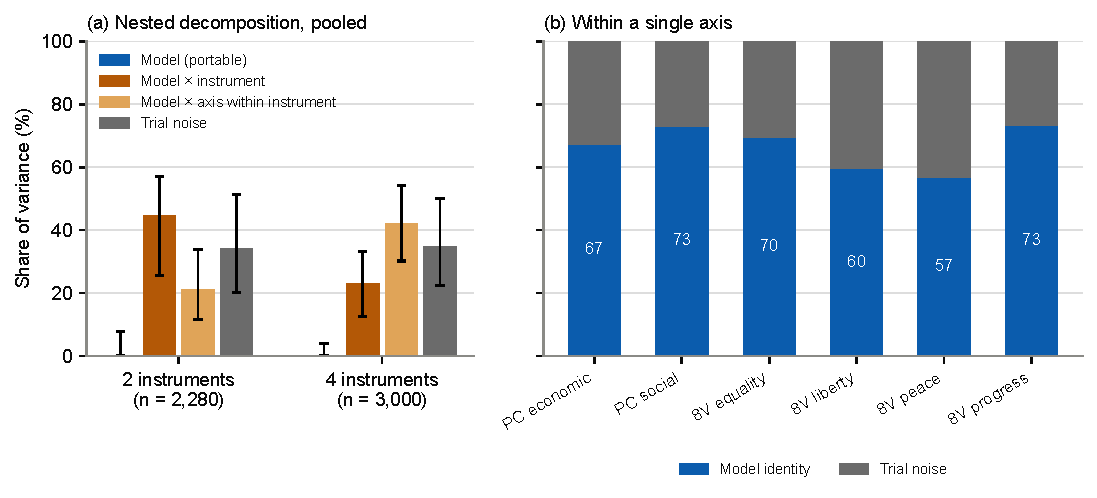
\includegraphics[width=\textwidth]{figures/fig_error_budget.pdf}
\caption{Variance components of a standardized political position (Equation~\ref{eq:model}). (a) Pooled shares with 95\%
bootstrap intervals for the two original instruments (19 models, 2,280 administrations) and for four instruments
(3,000 administrations). (b) Model-identity share within each axis. Same 0--100 vertical axis in both panels.}
\label{fig:budget}
\end{figure}

\begin{table}[H]
\centering
\caption{Variance shares (\%) of direction-aligned scores, with 95\% percentile intervals over models and over providers (1,000 resamples).
Two-instrument panel: 2,280 administrations, 19 models (July 2026); four-instrument panel: 3,000 administrations,
18 models on the added instruments (September 2026).}
\label{tab:budget}
\small
\begin{tabular}{llccc}
\toprule
Panel & Component & Share & CI, models & CI, providers \\
\midrule
Two instruments & Model (transfers) & 17.2 & [0.0, 40.0] & [0.0, 43.3] \\
 & Model $\times$ instrument & 27.7 & [11.5, 41.3] & [8.8, 37.9] \\
 & Model $\times$ axis(instrument) & 21.1 & [11.4, 34.0] & [10.5, 34.5] \\
 & Trial noise & 34.0 & [20.0, 50.7] & [19.9, 52.7] \\
\addlinespace
Four instruments & Model (transfers) & 2.0 & [0.0, 18.4] & [0.0, 18.8] \\
 & Model $\times$ instrument & 31.8 & [15.3, 40.7] & [14.4, 39.5] \\
 & Model $\times$ axis(instrument) & 31.3 & [19.0, 45.6] & [17.7, 47.4] \\
 & Trial noise & 34.9 & [22.2, 50.6] & [21.0, 52.3] \\
\bottomrule
\end{tabular}

\end{table}

The lean itself is not in question. All 114 model-axis cells differ from their instrument's midpoint (one-sample
$t$-tests, Benjamini--Hochberg false discovery rate 5\%), with a median standardized effect of 11.9 (95\% CI
[8.8, 16.7]). The midpoint is a convention, not a population estimate \citep{gallup2024values}.

\textbf{Convergent validity.} If instrument choice moves scores this much, one defence is that both instruments are
noisy measures of one position. The multitrait-multimethod analysis does not support it (Table~\ref{tab:mtmm}).
Convergent coefficients, the same construct on both instruments, average $r=\ConvMean$ ($SE=\ConvSE$, 95\% CI
\ConvCI); discriminant coefficients, different constructs on one instrument, average $r=\DiscMean$ ($SE=\DiscSE$).
The Campbell--Fiske criterion requires the first to exceed the second; it is lower by \DiffAbs{} ($SE=\DiffSE$, 95\% CI
\DiffCI). The two construct pairs differ. The social scales converge ($r=\ConvSoc$, $SE=\ConvSocSE$); the economic scales
do not ($r=\ConvEcon$, $SE=\ConvEconSE$). Averaged, the criterion fails; the social pair converges and the economic pair does not, and the economic estimate is too imprecise to rule out a correlation near 0.45. The estimate rests on two construct pairs and 19 models.

\begin{table}[H]
\centering
\caption{Multitrait-multimethod coefficients across 19 models (July 2026), Pearson $r$ of direction-aligned model means with
$SE(r)=\sqrt{(1-r^2)/(n-2)}$; means and difference with bootstrap SE over models.}
\label{tab:mtmm}
\small
\begin{tabular}{llrr}
\toprule
Type & Pair & $r$ & $SE$ \\
\midrule
Convergent & 8Values equality vs.\ Pol.\ Compass economic & $+0.005$ & 0.243 \\
Convergent & 8Values progress vs.\ Pol.\ Compass social & $+0.506$ & 0.209 \\
Discriminant & 8Values equality vs.\ 8Values progress & $+0.490$ & 0.211 \\
Discriminant & Pol.\ Compass economic vs.\ Pol.\ Compass social & $+0.549$ & 0.203 \\
\midrule
Mean convergent & & $+0.255$ & 0.165 \\
Mean discriminant & & $+0.520$ & 0.106 \\
Difference & & $-0.264$ & 0.140 \\
\bottomrule
\end{tabular}

\end{table}

SapplyValues locates the disagreement. Its economic axis agrees with 8Values equality on model ranking
($\rho=\RhoSapEq$, $SE=\RhoSapEqSE$) and disagrees with the Political Compass economic axis ($\rho=\RhoSapPC$,
$SE=\RhoSapPCSE$): of the three economic scales, the Political Compass's is the one that orders models differently. Pew's
ordinal position is unrelated to either ($\rho=\RhoPewPC$, $SE=\RhoPewPCSE$; $\rho=\RhoPewEq$, $SE=\RhoPewEqSE$).
Sixteen of 18 models classify left of centre on Pew's own typology, two (DeepSeek Chat, Grok 4.20) as \emph{Pragmatic and
Polite Right}.

\textbf{A positive control.} The instruments can agree. Every model answers further left for the progressive asker than
for the conservative one on every axis of both instruments (\KGPositive{} of \KGCells{} model--axis cells), by
\KGRangeLo--\KGRangeHi\% of the instrument's range, or \KGSdLo--\KGSdHi{} times the spread between models with no asker.
The size of a model's shift on one instrument tracks its shift on the other (mean convergent $r=\KGShift$, 95\% CI
\KGShiftCI), against $r=\KGBase$ (\KGBaseCI) for the same models' no-asker positions in that design. Both questionnaires
register a large common signal alike; what fails to transfer is the far smaller difference between models' default
positions.

\textbf{Robustness.} Dropping each provider in turn from the four-instrument panel leaves the nested transferable
share between \LopoMmin\% and \LopoMmax\%. Dropping each instrument leaves it between \LoioMmin\% and \LoioMmax\%, while
the instrument-specific share ranges from \LoioMImin\% to \LoioMImax\% and the axis-specific share from \LoioMAmin\%
to \LoioMAmax\%: the data show that little transfers across questionnaires more firmly than they apportion the rest
between instrument and axis. I therefore claim that a model's position depends on instrument and axis jointly. Two axes have no settled left--right polarity (8Values peace,
SapplyValues authority); reversing either or both puts the four-instrument transferable share between \OrientFourMin\%
and \OrientFourMax\%, and reversing 8Values peace puts the two-instrument share at \OrientTwoMax\% rather than \NTwoM\%, because that reversal moves variance from the instrument term to the axis term (Online Appendix). A
re-administration of 8Values at temperatures 0 and 1.0 to eight models (20 trials each) finds trial noise rising from
24\% to 31\% (0.7) to 47\% of variance while model rankings stay stable (mean Spearman 0.88--0.92): the noise share is
conditional on temperature. A second and third language-model judge reproduce the open-ended arm's scores closely
(Spearman 0.85--0.92), which is agreement among models, not validation against human raters (Online Appendix).

\textbf{Three further factors.} In their own designs, asker identity explains more variance than model identity (partial
$\eta^2$ 0.77--0.84 across the six axes, mean 0.79, against 0.16--0.35, mean 0.23); accommodation is asymmetric, moving
scores 2.9--6.7 times further from baseline for a conservative framing than a progressive one, on top of a baseline that
already leans left. Sense-inverting items with the scoring key flipped yields a Contamination Index averaging 0.046 of
the instrument's range (95\% CI [0.038, 0.055]), with 17 of 18 models shifting on at least one axis after correction;
the memorisation probe finds 16.6\% verbatim and 20.6\% near-verbatim completions. Free-text versus forced-label
elicitation explains more variance on average (0.39 against 0.23), though not on every axis: on 8Values equality model
identity is larger (0.42 against 0.06). Each factor was collected as its own factorial rather than crossed with instrument,
so these designs cannot be added into one budget, and I do not estimate how a single crossed design would change the
model share.

\textbf{Item-level reliability.} Measured per item, 44.8\% of model--item cells are perfectly stable across all 60
repetitions, and the most volatile decile of items carries under 16\% of response entropy on either instrument:
inconsistency is concentrated in a minority of contested items. A range-normalized stability metric used in earlier work
assigns one of the worst instability scores to a model whose answers varied by six hundredths of a point; any scale-free
consistency statistic that divides by observed spread inverts on tightly clustered responses, which is why I use a
variance-components estimate. A graded-response item-response analysis shows that some apparent centrism is avoidance: the
most neutral model answers 52\% of 8Values items at the midpoint against 9\% for the least.

\section{Discussion}

The finding that models lean left reproduces here as elsewhere. What this paper adds is a denominator. Between half and
two-thirds of a score depends on the instrument and axis. The share that carries across instruments is estimated at
\NFourMr\% to \NTwoMr\% depending on which instruments are used, with intervals that include zero, and repetition
alone contributes more than that point estimate. The lean survives, but most of the variation in a reported lean is not
a property of the model that carries beyond the instrument used. That matters because the field's
quantitative claims are magnitude claims: that one model is more partisan than another, that alignment shifts a model by
some amount, or that lean has grown across generations all require scores comparable across studies, and the two most
widely used instruments converge on the social scale only. The failure is one of transportability, not of auditing:
within a single instrument model identity is clearly measurable, and both instruments register a change of asker
alike. The remedy has precedent in this literature, where a single
output is not safe to treat as a measurement without characterizing how it fails \citep{bisbee2024}.

I do not claim that a questionnaire score predicts behaviour. A study comparing a voting-advice questionnaire with real
referendum outcomes finds models near the centre on concrete votes despite a left-leaning profile on the questionnaire
\citep{barmettler2026instrument}; that is a behavioural-validity question this design does not test. The limits are
real: English-language administrations on US-built instruments at one time point; 19 models from 11 providers are a small
sample of a population of models; the main design used one temperature and one prompt wrapper; the direction alignment
treats left, libertarian and progressive as one pole, which is the direction of the models' common lean but a convention;
and the language-model judges were not validated against humans.

\textbf{A minimum reporting standard.} A political-bias audit of a language model should report: the instrument, named,
with its items; the asker condition, including the absence of one, since an unattributed prompt is a condition, not a
neutral baseline; repetition count and dispersion in the instrument's units; an error budget or at least a variance
decomposition across whatever was varied; the model version, route, date and sampling settings, with raw outputs
archived; a contamination check; and item-level results. The same logic applies to any study that treats a language
model's answers to a survey scale or coding scheme as a measure \citep{argyle2023, serapiogarcia2023}: the instrument
is a random facet, one instrument confounds model identity with instrument-specific position, and repetition is
required. Researchers who position texts or respondents with a model face the same choice of prompt wrapper and scoring
rule, which is the validation stage \citet{lemens2025asking} advise readers not to skip. Adopting even the first few
items would make the existing literature's estimates comparable, which at present they mostly are not.

\textbf{Use of generative AI.} A commercial generative AI assistant was used interactively to draft and revise parts of
the prose and to write and refactor the collection, scoring, analysis and figure code. It generated no data. The author
verified its output, re-derived every reported number from the archived raw trials with the released scripts in a clean
environment, and is responsible for the content; the tool and dates are named on the title page.

\textbf{Replication.} All raw trials, scoring adapters and analysis code reproduce every number reported here offline
without API access; collection itself cannot be re-run identically. The archive and its data citation are given on the title
page and will be deposited in the journal's Dataverse on acceptance.

\clearpage
\bibliographystyle{agsm}
\bibliography{references}

\end{document}
